\documentclass[12pt,a4paper]{article}
\usepackage{fontspec}
\defaultfontfeatures{Mapping=tex-text}
\usepackage{xunicode}
\usepackage{xltxtra}
%\setmainfont{???}
\usepackage{polyglossia}
\usepackage{halloweenmath}
\usepackage{csquotes}
\usepackage{graphicx}
\usepackage{hyperref}
\usepackage{stmaryrd}
\usepackage{qtree}
\usepackage{gb4e}
\setdefaultlanguage{english}
\author{Katrina Olsen}
\title{Moses Illusion Report}
\begin{document}
\maketitle

\tableofcontents

\section{Moses Illusion}
Moses illusions are cases where a speaker answers a question using common knowledge, even though the question itself is nonsensical and merely similar to a common question.
\subsection{Moses Example} \label{mosex}
\textbf{Common Knowledge Question:} \enquote{How many of each animal did Noah take on the arc?}\\
\textbf{Correct Answer:} 2\\
\\
\textbf{Moses Illusion Question:} \enquote{How many of each animal did Moses take on the arc?}\\
\textbf{Moses Illusion Answer:} 2\\
\textbf{Correct Answer:} \enquote{can't answer} / \enquote{NA} / etc.
\section{Experiment}
\subsection{Methods}
The data was collected via an online survey in April 2024.
\subsubsection{Participants}
The participants of the study were the students attending the Digital Research Toolkit for Linguistics course in the Summer Semester of 2024 at the University of Stuttgart. The students were invited to invite friends and family to participate as well.

\subsubsection{Materials}
The experiment's materials followed that of Erickson \& Mattson 1981. Their research and this experiment were both run in English, however this experiment could be performed in any other language.
\begin{exe}
\ex
\gll Wie viele Zahlen hat das deutsche Alphabet?\\
how many number.pl has the german.fem alphabet\\
\glt How many numbers are in the German alphabet?
\end{exe}
% I did this going from another language into English, I hope that's okay. English is my native language, so I didn't know what to do

The questions follow many various syntactic structures that could be represented in trees. However, once seeing the syntax command \enquote{roof}, the author of this paper really wanted to put a math witch flying over one.


\Tree [.S [.NP [.Det This ] [.N \mathwitch* ] ] [.VP [.VP [.V flies ] ] [.PP [.P over ] [.NP \qroof{this house}.NP [.Cor and ] \qroof{this house}.NP ] ] ] ]

\vspace{1em}
However, in case the trees have to be related to the data, here is a tree representing one of the common response's syntax.
\vspace{1em}

\Tree [.S [.NP -NONE- ] [.VP [.Modal can ] [.VP [.Neg 't ] [.VP [.V answer ] ] ] ] ]

\vspace{1em}
The semantics of being correct in this study can be understood as: $\forall x^s (know(x^s, answer) \rightarrow correct(x^s)$.

% Sorry if the trees or semantics are nonsensically incorrect, it's been a really long time since I've done these


\subsubsection{Procedure}
The survey began with instructions for the participant to read each question and spontaneously answer either: \enquote{don't know} if they didn't know, or \enquote{can't answer} if the question is \enquote{distorted or nonsensical}. The instructions also provided an example question for each of these potential answer types.
\subsection{Predictions} \label{predic}
Following the previous research done by Erickson \& Mattson 1981, it was expected that some participants would not answer every Moses illusion question with "can't answer", even though they were told there would be nonsensical questions in the instructions.
\subsection{Data Labeling}
The experiments were run on Moses Illusion questions, normal common knowledge questions, and control questions. All submitted answers were given the following labels:
\begin{itemize}
  \item Correct
  \item Incorrect
  \item Don't Know
\end{itemize}
The labels were assigned according the the answer and question types. Using the Moses Illusion and Common Knowledge example questions discussed in Section \ref{mosex} as an example, the participants' answers would be labeled as in Table \ref{tab:ex}.

\begin{table}
    \centering
    \begin{tabular}{ccc}
        \textbf{Question Type} & \textbf{Answer} & \textbf{Label}\\
        Common Knowledge & 2 & Correct\\
        Common Knowledge & 1 & Incorrect\\
        Moses Illusion & 2 & Incorrect\\
        Moses Illusion & can't answer & Correct\\
    \end{tabular}
    \caption{Labeling Method per Question Type}
    \label{tab:ex}
\end{table}

\section{Analysis and Results}
\begin{figure}
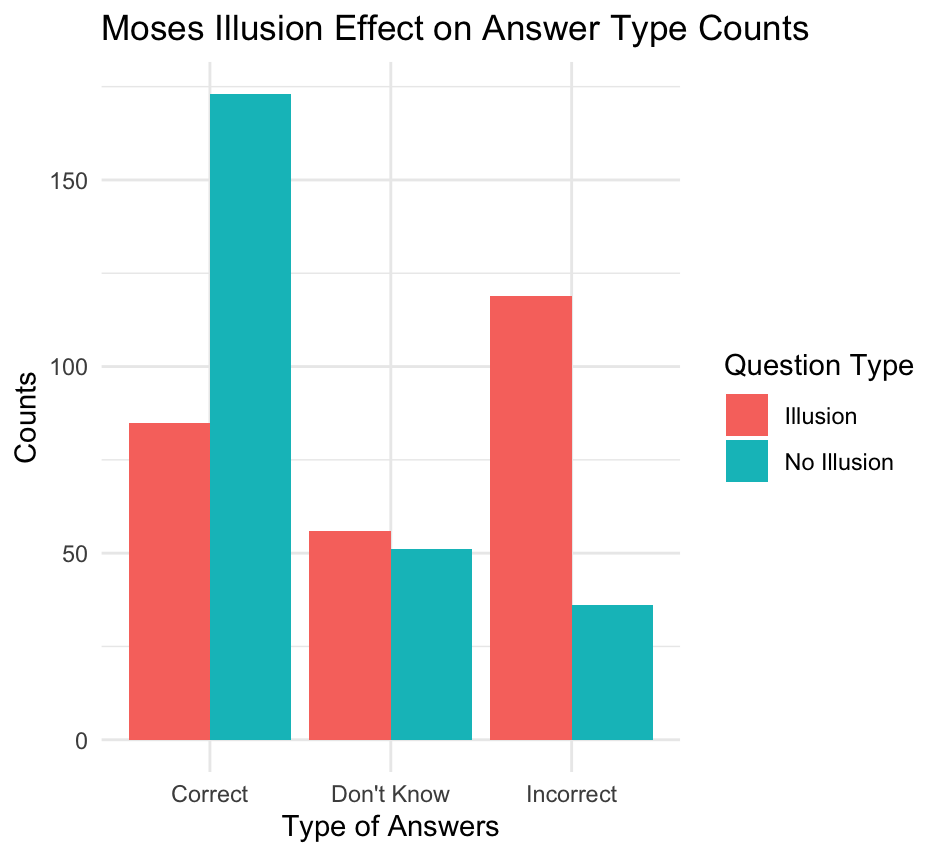
\includegraphics
[width=1\textwidth]{MosesIllusionEffect.png}
\caption{Count of each answer type for questions with and without the Moses Illusion}\label{fig:effect}
\end{figure} 
As seen in Figure \ref{fig:effect}, the predictions stated in Section \ref{predic} proved true. The number of incorrect answers increases significantly on Moses illusion questions.
\section{References}
Erickson, Thomas D and Mark E Mattson (1981). “From words to
meaning: A semantic illusion”. In: Journal of Verbal Learning and
Verbal Behavior 20.5, pp. 540–551. DOI:
10.1016/s0022-5371(81)90165-1.

\end{document}